\documentclass [11pt,twoside]{article}

\newcommand{\names}{Manuel Pedrozo, Tomás Perez Molina}
\newcommand{\projectName}{SafeStreets}

\usepackage[utf8]{inputenc}
\usepackage[T1]{fontenc}

%Page margins, header and footer positions
\usepackage{geometry}
 \geometry{
 a4paper,
 total={210mm,297mm},
 left=25mm,
 right=25mm,
 top=30mm,
 bottom=25mm,
 headsep=7mm}

\interfootnotelinepenalty=10000

%To display filling dots in the TOC for all entries
\usepackage[titles]{tocloft}
\renewcommand{\cftsecleader}{\cftdotfill{\cftdotsep}}

%Define new header and footer style
\usepackage{fancyhdr}

\pagestyle{fancy}
\fancyhf{}
\lhead{\color{Gray}{\small{\projectName{} project by \names{}}}}
\lfoot{\textcolor{Gray}{\small{Copyright © 2019, \names{} – All rights reserved}}}
\rfoot{\textcolor{Gray}{\thepage}}
\renewcommand{\headrulewidth}{0pt}

%PACKAGES
\usepackage{wasysym}
\usepackage{pifont}

\newcommand{\supported}{\ding{52}\xspace}
\newcommand{\unsupported}{\ding{55}\xspace}
\newcommand{\partsupported}{\textcolor{black!40}{\ding{52}}\xspace}
\newcommand{\lowsupported}{\textcolor{black!20}{\ding{52}}\xspace}
\newcommand{\unknowsupported}{\textbf{?}\xspace}

%Font: Times
\usepackage{times}
%Change monospaced font
\renewcommand{\ttdefault}{lmtt}

%tables
\usepackage{tabu}
\usepackage{tabularx}
\usepackage{ltablex}
\usepackage{longtable}
\usepackage{float} % To allow the use of H modifier in long tables

%landscape mode
\usepackage{pdflscape}
\usepackage{rotating}
\usepackage{caption}

%make landscape mode be sensitive to even and odd pages
%start
\def\myrotate{\ifodd\c@page\else-\fi 90}
\makeatletter
\global\let\orig@begin@landscape=\landscape%
\global\let\orig@end@landscape=\endlandscape%
\gdef\@true{1}
\gdef\@false{0}
\gdef\landscape{%
    \global\let\within@landscape=\@true%
    \orig@begin@landscape%
}%
\gdef\endlandscape{%
    \orig@end@landscape%
    \global\let\within@landscape=\@false%
}%
\@ifpackageloaded{pdflscape}{%
    \gdef\pdf@landscape@rotate{\PLS@Rotate}%
}{
    \gdef\pdf@landscape@rotate#1{}%
}
\let\latex@outputpage\@outputpage
\def\@outputpage{
    \ifx\within@landscape\@true%
        \if@twoside%
            \ifodd\c@page%
                \gdef\LS@rot{\setbox\@outputbox\vbox{%
                    \pdf@landscape@rotate{-90}%
                    \hbox{\rotatebox{90}{\hbox{\rotatebox{180}{\box\@outputbox}}}}}%
                }%
            \else%
                \gdef\LS@rot{\setbox\@outputbox\vbox{%
                    \pdf@landscape@rotate{+90}%
                    \hbox{\rotatebox{90}{\hbox{\rotatebox{0}{\box\@outputbox}}}}}%
                }%
            \fi%
        \else%
            \gdef\LS@rot{\setbox\@outputbox\vbox{%
                \pdf@landscape@rotate{+90}%
                \hbox{\rotatebox{90}{\hbox{\rotatebox{0}{\box\@outputbox}}}}}%
            }%
        \fi%
    \fi%
    \latex@outputpage%
}
\makeatother
%end

%graphics
\usepackage{graphicx}
\usepackage[dvipsnames, table]{xcolor}
%If you upload images from PC, you need to insert code for the path here (different for Windows and Unix OS)

%References
%\usepackage{xpatch}
%\usepackage[backend=biber, style=numeric, citestyle=numeric, sorting=none]{biblatex}
%\addbibresource{main.bib}

%Other
\usepackage{ifthen}
\usepackage{xspace}
\usepackage{enumitem}
\usepackage{amssymb}
\usepackage[pdftex, colorlinks]{hyperref}
\newcommand{\comment}[1]{{\color{Red}$\blacktriangleright$ Comment: #1 $\blacktriangleleft$}}


% Some utilities\ldots
\usepackage{soul}
\usepackage{tikz}

\usetikzlibrary{calc}
\usetikzlibrary{decorations.pathmorphing}


\makeatletter

\newcommand{\defhighlighter}[3][]{%
  \tikzset{every highlighter/.style={color=#2, fill opacity=#3, #1}}%
}

\defhighlighter{yellow}{.5}

\newcommand{\highlight@DoHighlight}{
  \fill [ decoration = {random steps, amplitude=1pt, segment length=15pt}
        , outer sep = -15pt, inner sep = 0pt, decorate
       , every highlighter, this highlighter ]
        ($(begin highlight)+(0,8pt)$) rectangle ($(end highlight)+(0,-3pt)$) ;
}

\newcommand{\highlight@BeginHighlight}{
  \coordinate (begin highlight) at (0,0) ;
}

\newcommand{\highlight@EndHighlight}{
  \coordinate (end highlight) at (0,0) ;
}

\newdimen\highlight@previous
\newdimen\highlight@current

\DeclareRobustCommand*\highlight[1][]{%
  \tikzset{this highlighter/.style={#1}}%
  \SOUL@setup
  %
  \def\SOUL@preamble{%
    \begin{tikzpicture}[overlay, remember picture]
      \highlight@BeginHighlight
      \highlight@EndHighlight
    \end{tikzpicture}%
  }%
  %
  \def\SOUL@postamble{%
    \begin{tikzpicture}[overlay, remember picture]
      \highlight@EndHighlight
      \highlight@DoHighlight
    \end{tikzpicture}%
  }%
  %
  \def\SOUL@everyhyphen{%
    \discretionary{%
      \SOUL@setkern\SOUL@hyphkern
      \SOUL@sethyphenchar
      \tikz[overlay, remember picture] \highlight@EndHighlight ;%
    }{%
    }{%
      \SOUL@setkern\SOUL@charkern
    }%
  }%
  %
  \def\SOUL@everyexhyphen##1{%
    \SOUL@setkern\SOUL@hyphkern
    \hbox{##1}%
    \discretionary{%
      \tikz[overlay, remember picture] \highlight@EndHighlight ;%
    }{%
    }{%
      \SOUL@setkern\SOUL@charkern
    }%
  }%
  %
  \def\SOUL@everysyllable{%
    \begin{tikzpicture}[overlay, remember picture]
      \path let \p0 = (begin highlight), \p1 = (0,0) in \pgfextra
        \global\highlight@previous=\y0
        \global\highlight@current =\y1
      \endpgfextra (0,0) ;
      \ifdim\highlight@current < \highlight@previous
        \highlight@DoHighlight
        \highlight@BeginHighlight
      \fi
    \end{tikzpicture}%
    \the\SOUL@syllable
    \tikz[overlay, remember picture] \highlight@EndHighlight ;%
  }%
  \SOUL@
}

\makeatother

% Common abbrev. are set as commands to ensure proper spacing after the dot
\RequirePackage{xspace}
\newcommand{\ie}{i.e.\@\xspace}
\newcommand{\aka}{a.k.a.\@\xspace}
\newcommand{\Ie}{I.e.\@\xspace}
\newcommand{\cf}{cf.\@\xspace}
\newcommand{\Cf}{Cf.\@\xspace}
\newcommand{\eg}{e.g.\@\xspace}
\newcommand{\Eg}{E.g.\@\xspace}
\newcommand{\etal}{et al.\@\xspace}
\newcommand{\etc}{etc.\@\xspace}
\newcommand{\wrt}{w.r.t.\@\xspace}
\newcommand{\Wrt}{W.r.t.\@\xspace}



\date{}
\raggedbottom

\usepackage[dvipsnames]{xcolor}
\usepackage{listings}


\begin{document}

%TITLE PAGE

\begin{titlepage}


%LOGO

{\begin{table}[t!]
\centering
\begin{tabu} to \textwidth { X[1.3,r,p] X[1.7,l,p] }
\textcolor{Blue}
{\textbf{\small{\projectName{} project \newline \names{}}}} & 
\includegraphics[scale=0.5]{Images/PolimiLogo}
\end{tabu}
\end{table}}~\\ [7cm]

%TITLE 

\begin{flushleft}

%Replace the text string with your title
{\textcolor{Blue}{\textbf{\Huge{Implementation and Testing Deliverable}}}} \\ [1cm]

\end{flushleft}

\vspace{9cm}
\begin{itemize}[label={{}}]  \itemsep0em
        \item Source code: \url{https://github.com/lethanity/PedrozoPerez/tree/master/implementation}
        \item Installation: \url{https://github.com/lethanity/PedrozoPerez/tree/master/DeliveryFolder/implementation}
\end{itemize}

\end{titlepage}

%Define deliverable specific info
%Replace cell contents where needed
\begin{table}[h!]
\begin{tabu} to \textwidth { X[0.3,r,p] X[0.7,l,p] }
\hline

\textbf{Deliverable:} & ITD\\
\textbf{Title:} & Implementation and Testing Deliverable \\
\textbf{Authors:} & \names{} \\
\textbf{Version:} & 1.0 \\ 
\textbf{Date:} & \today \\
\textbf{Download page:} & \url{https://github.com/lethanity/PedrozoPerez} \\
\textbf{Copyright:} & Copyright © 2020, \names{}  – All rights reserved \\
\hline
\end{tabu}
\end{table}




\setcounter{page}{2}


%------------------------------------------------------------------------------------------------------------------------------------------------
\newpage
\addcontentsline{toc}{section}{Table of Contents}
\tableofcontents
\newpage
\addcontentsline{toc}{section}{List of Figures}
\listoffigures
\addcontentsline{toc}{section}{List of Tables}
\listoftables

%------------------------------------------------------------------------------------------------------------------------------------------------
\clearpage
{\color{Blue}{\section{Introduction}}}
\label{sect:introduction}
This document has been prepared to help you approaching Latex as a formatting tool for your Travlendar+ deliverables. This document suggests you a possible style and format for your deliverables and contains information about basic formatting commands in Latex. A good guide to Latex is available here \href{https://tobi.oetiker.ch/lshort/lshort.pdf}{https://tobi.oetiker.ch/lshort/lshort.pdf}, but you can find many other good references on the web. 

Writing in Latex means writing textual files having a \texttt{.tex} extension and exploiting the Latex markup commands for formatting purposes. Your files then need to be compiled using the Latex compiler. Similarly to programming languages, you can find many editors that help you writing and compiling your latex code. Here \href{https://beebom.com/best-latex-editors/}{https://beebom.com/best-latex-editors/} you have a short oviewview of some of them. Feel free to choose the one you like.  

Include a subsection for each of the following items\footnote{By the way, what follows is the structure of an itemized list in Latex.}:
\begin{itemize}
\item
Purpose: here we include the goals of the project
\item
Scope: here we include an analysis of the world and of the shared phenomena
\item
Definitions, Acronyms, Abbreviations
\item
Revision history
\item
Reference Documents 
\item
Document Structure
\end{itemize}
Below you see how to define the header for a subsection.
\subsection{Scope}
... Here you see a subsubsection
\subsubsection{World Phenomena}
%what you write here is a comment that is not shown in the final text

%------------------------------------------------------------------------------------------------------------------------------------------------
\clearpage
{\color{Blue}{\section{Implemented requirements}}}
\label{sect:requirements}
Organize this section according to the rules defined in the project description. 


%------------------------------------------------------------------------------------------------------------------------------------------------
\clearpage
{\color{Blue}{\section{Adopted development frameworks}}}
\label{sect:frameworks}
Since the development time for the application is short, for the most part the team opted for known technologies as to reduce the risk of missing the timeline by encountering unexpected obstacles. This also allowed the team to focus on unknown areas, like the integration with external APIs.\\

\subsection{Mobile}
As stated in section 5.1.1 of the Design Document, the mobile application is developed in the Flutter framework, which uses the Dart programming language.
The advantage of Flutter is that it is a complete toolset, allowing for development without the necessity of third party packages for core functionality, which can bring incompatibilities. In spite of that, some packages more specific to the application were used to speed up development (such as the map, geolocation and camera). Also, being completely written in Dart, a typed language, makes implementation more intuitive and easier to follow compared to web technologies, which juggle HTML, CSS and Javascript at the same time.
The main disadvantage of Flutter is, at the same time, the Dart language which is very young (2013) and unknown to most developers currently. However, its syntax is familiar and easy to pickup.

\subsection{Back-end server}

As stated in section 5.1.2 of the Design Document, the backend is implemented in Kotlin utilizing the Spring boot framework.
Kotlin was chosen over Java because its more concise, safer and allows for faster development for those familiar with it.
Spring is one of the most popular frameworks for the development of web applications, based on the JVM. It allows for fast development and easy integration with documentation tools that help speed up the work. Because of its maturity and popularity, there is a great amount of documentation on the framework itself. There are a few alternatives, like Play and Grails, which offer similar functionalities, but Spring has been proven to be the most performant of the three.


%------------------------------------------------------------------------------------------------------------------------------------------------
\clearpage
{\color{Blue}{\section{Structure of the source code}}}
\label{sect:sourcecode}
\subsection{Back-end server}
The source code is organized following the Gradle standard.\\

The application resides in the /back directory, where Gradle configuration files can be found.

\begin{itemize}
    \item 
    /src
    \begin{itemize}[label={$\diamond$}]
        \item 
        /main \textcolor{black!70}{contains the source code files.}
        \item 
        /java/com/openalpr/jni \textcolor{black!70}{contains the OpenALPR java files.}
        \item 
        /kotlin/se2/SafeStreets/back \textcolor{black!70}{contains the kotlin files, organized according to Spring boot framework.}
        \begin{itemize}[label={\textbf{-}}]
            \item 
            /controller \textcolor{black!70}{contains Spring controller classes.}
            \item 
            /model \textcolor{black!70}{contains application models and DTOs.}
            \item 
            /repository \textcolor{black!70}{contains Spring repository classes.}
            \item 
            /security \textcolor{black!70}{contains Spring security configuration and filters.}
            \item 
            /service \textcolor{black!70}{contains Spring service classes.}
        \end{itemize}
        \item 
        /resources \textcolor{black!70}{contains resources used by the application, like Spring properties files.}
    \end{itemize}

    \item 
    /test \textcolor{black!70}{contains the source code files for testing.}
    \begin{itemize}[label={$\diamond$}]
        \item 
        /kotlin/se2/SafeStreets/back \textcolor{black!70}{contains unit test classes.}
        \item 
        /resources \textcolor{black!70}{contains files used for testing, like images.}
    \end{itemize}
\end{itemize}


%------------------------------------------------------------------------------------------------------------------------------------------------
\clearpage
{\color{Blue}{\section{Testing}}}
\label{sect:testing}
The acceptance tests performed are based on the documentation provided by the team. \\

\subsection{Acceptance tests based on use cases}
The tests were developed taking the use cases described in the RASD and modifying them according to what was finally implemented as explained in the ITD. 
The “expected steps” describe the flow we would expect to follow to complete a test, before coming into contact with the finished prototype. While the “real steps” are the steps followed to complete the use case when using the prototype. \\

\begin{table}[H]
    \centering
    \begin{tabular}{p{3cm}p{10cm}}
    \textbf{Test ID} & AT-001-SIGN\_UP \\ \hline
    \textbf{Based on} & Registration as a Normal User to SafeStreets \\ \hline
    \textbf{Pre-requisites} & - \\ \hline
    \textbf{Expected steps} & 
        \begin{enumerate} \itemsep0em
            \item The System shows the registration page.
            \item Input the following data: email, name, surname and password.
            \item Agree to the privacy policy of SafeStreets.
            \item Confirm and send the form.
            \item Receive a confirmation email to the email provided.
            \item Confirm email account following the provided link.
            \item The user is registered and logged in and is redirected to the home page.
        \end{enumerate} \\ \hline
    \textbf{Real steps} & 
        \begin{enumerate} \itemsep0em
            \item The system shows the registration page.
            \item Fill the form with the following data:
                \begin{itemize}[label={}] \itemsep0em
                    \item Name: Robert
                    \item Surname: Jones
                    \item Email: robert@mail.com
                    \item Password: robert123
                \end{itemize}
            \item Press the Sign Up button.
            \item The user is registered and logged in and the system shows the home page.
        \end{enumerate} \\ \hline
    \textbf{Expected output} & User correctly registered and redirected to the home page. \\ \hline
    \textbf{Outcome} & Success \\ \hline
    \textbf{Alternative flow} & 
        \begin{itemize} \itemsep0em
            \item In step 4, if any field form is either empty or invalid, the message “Wrong data, impossible to sign up” is shown.
        \end{itemize} \\ \hline
    \end{tabular}
\end{table}

\begin{table}[H]
    \centering
    \begin{tabular}{p{3cm}p{10cm}}
    \textbf{Test ID} & AT-002-REPORT\_VIOLATION \\ \hline
    \textbf{Based on} & Violation report sent by User to SafeStreets \\ \hline
    \textbf{Pre-requisites} & Logged into the app \\ \hline
    \textbf{Expected steps} & 
        \begin{enumerate} \itemsep0em
            \item Select the camera.
            \item The system shows the camera screen.
            \item Press the button or screen to take a picture of the violation.
            \item The system shows the form to add the type of violation.
            \item Select a type of violation.
            \item Confirm the license plate recognized by the system.
            \item Press the button to send the report.
            \item The system shows the home screen.
        \end{enumerate} \\ \hline
    \textbf{Real steps} & 
        \begin{enumerate} \itemsep0em
            \item Press the camera button.
            \item The system shows the camera screen.
            \item Press the button to take a picture of a car.
            \begin{itemize}[label={}] \itemsep0em
                \item Picture:
                \item 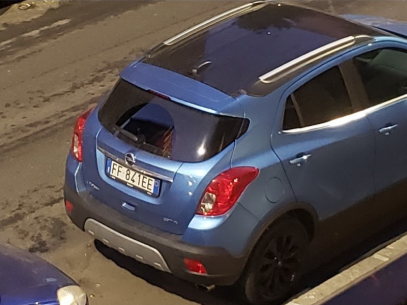
\includegraphics[width=.3\textwidth]{Images/test-photo.png}
            \end{itemize}
            \item The system shows a form to add a license plate and select a type of violation.
            \item Enter the car license plate: FF841EE
            \item Select parking violation.
            \item Press the button to send the report.
            \item The system shows a screen with a “Report sent successfully, thanks for your contribution” message.
        \end{enumerate} \\ \hline
    \textbf{Expected output} & Report submitted, app redirects to home page. \\ \hline
    \textbf{Real output} & Report submitted successfully, confirmed by a notification. App redirects to thank you message. \\ \hline
    \textbf{Outcome} & Partial success, core functionality is working but does not redirect to the home screen as indicated in the RASD. \\ \hline
    \textbf{Alternative flow} & 
        \begin{itemize} \itemsep0em
            \item Backing out of taking a picture after step 2 results in a continuous loading indicator displaying “Taking picture…”.
        \end{itemize} \\ \hline
    
    \end{tabular}
\end{table}

\begin{table}[H]
    \centering
    \begin{tabular}{p{3cm}p{10cm}}
        \textbf{Notes} & The system does not appear to detect license plates in a photo, as the license plate input is always shown.
        Other photos used:
        
\includegraphics[width=.3\textwidth]{Images/test-photo2.png}
        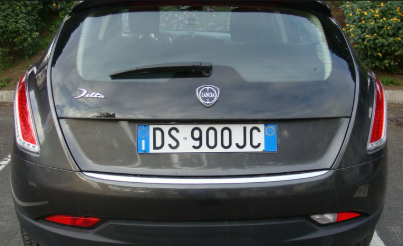
\includegraphics[width=.3\textwidth]{Images/test-photo3.png}
     \\ \hline
    \end{tabular}
\end{table}

\begin{table}[H]
    \centering
    \begin{tabular}{p{3cm}p{10cm}}
    \textbf{Test ID} & AT-003-REPORT\_HISTORY \\ \hline
    \textbf{Based on} & History report requested by User. \\ \hline
    \textbf{Pre-requisites} & Logged into the app. \\ \hline
    \textbf{Expected steps} & 
        \begin{enumerate} \itemsep0em
            \item Select the report history.
            \item The system shows the report history.
        \end{enumerate} \\ \hline
    \textbf{Real steps} & 
        \begin{enumerate} \itemsep0em
            \item Press the “Get My Report” button.
            \item The system shows the report history.
        \end{enumerate} \\ \hline
    \textbf{Expected output} & The report history is displayed on the screen. \\ \hline
    \textbf{Outcome} & Success \\ \hline
    \end{tabular}
\end{table}

% TODO
\begin{table}[H]
    \centering
    \begin{tabular}{p{3cm}p{10cm}}
    \textbf{Test ID} & AT-004-CHECK\_LICENSE\_PLATE\_VIOLATIONS \\ \hline
    \textbf{Based on} & Checking license plate violations by an Authority. \\ \hline
    \textbf{Pre-requisites} & Logged into the app as an Authority. \\ \hline
    \textbf{Expected steps} & 
        \begin{enumerate} \itemsep0em
            \item Input the license plate code.
            \item The system displays a list of reports for the given license plate ordered by date in descending order.
        \end{enumerate} \\ \hline
    \textbf{Real steps} & 
        \begin{enumerate} \itemsep0em
            \item aaaaa
            \item aaaaa
            \item aaaaa
            \item aaaaa
            \item aaaaa
        \end{enumerate} \\ \hline
    \textbf{Expected output} & The list of reports for the given license plate is displayed. \\ \hline
    \textbf{Real output} &  \\ \hline
    \textbf{Outcome} & Success \\ \hline
    \end{tabular}
\end{table}

\begin{table}[H]
    \centering
    \begin{tabular}{p{3cm}p{10cm}}
    \textbf{Test ID} & AT-005-VIOLATION\_NOTIFICATION \\ \hline
    \textbf{Based on} & Real-time notification about nearby violation for an Authority. \\ \hline
    \textbf{Pre-requisites} & Logged into the app as an Authority with the notification service activated. \\ \hline
    \textbf{Expected steps} & 
        \begin{enumerate} \itemsep0em
            \item Submit a report with another phone in close proximity
            \item Receive a notification.
            \item Press the notification message.
            \item The system displays the report, providing the exact location of the report.
        \end{enumerate} \\ \hline
    \textbf{Real steps} & 
        \begin{enumerate} \itemsep0em
            \item Subscribe to notifications for all areas available on the settings screen.
            \item Receive a notification.
            \item System displays a message stating that a new violation was reported in the area.
        \end{enumerate} \\ \hline
    \textbf{Expected output} & The system displays the report with its exact location. \\ \hline
    \textbf{Real output} & The system displays a message indicating the area of the report. \\ \hline
    \textbf{Outcome} & Partial fail, the notifications work but they do not display either the report nor its exact location. \\ \hline
    \textbf{Alternative flow} & 
        \begin{itemize} \itemsep0em
            \item If the app is not open, a system notification pop ups, but when pressed it just opens the app on the screen it was on. If the app was completely closed, it opens it on the home screen.
        \end{itemize} \\ \hline
    \end{tabular}
\end{table}


\begin{table}[H]
    \centering
    \begin{tabular}{p{3cm}p{10cm}}
    \textbf{Test ID} & AT-006-LIST\_AREA\_VIOLATIONS \\ \hline
    \textbf{Based on} & List of violations in an area for an Authority. \\ \hline
    \textbf{Pre-requisites} & Logged into the app as an Authority. \\ \hline
    \textbf{Expected steps} & 
        \begin{enumerate} \itemsep0em
            \item Input the area of interest.
            \item The system shows a list of reports in the area.
        \end{enumerate} \\ \hline
    \textbf{Real steps} & 
        \begin{enumerate} \itemsep0em
            \item aaaaa
            \item aaaaa
            \item aaaaa
            \item aaaaa
            \item aaaaa
        \end{enumerate} \\ \hline
    \textbf{Expected output} & The system displays a list of reports inside the given area. \\ \hline
    \textbf{Real output} &  \\ \hline
    \textbf{Outcome} & aaaaa \\ \hline
    \end{tabular}
\end{table}

\subsection{Other acceptance tests}
Taking into account the functionality implemented, further acceptance tests were performed. However, as there were no use cases for these, there are no expected steps to perform. \\

\begin{table}[H]
    \centering
    \begin{tabular}{p{3cm}p{10cm}}
    \textbf{Test ID} & AT-007-SIGN\_IN \\ \hline
    \textbf{Pre-requisites} & User already signed up to the system. \\ \hline
    \textbf{Real steps} & 
        \begin{enumerate} \itemsep0em
            \item Fill the sign in form with the following data:
            \begin{itemize}[label={}] \itemsep0em
                \item Email: robert@mail.com
                \item Password: robert123
            \end{itemize}
            \item Press the sign in button.
        \end{enumerate} \\ \hline
    \textbf{Expected output} & The system displays the home screen. \\ \hline
    \textbf{Real output} & The system displays the home screen. \\ \hline
    \textbf{Outcome} & Success \\ \hline
    \end{tabular}
\end{table}

\begin{table}[H]
    \centering
    \begin{tabular}{p{3cm}p{10cm}}
    \textbf{Test ID} & AT-009-AREA\_SAFETY \\ \hline
    \textbf{Pre-requisites} & Logged into the application. \\ \hline
    \textbf{Real steps} & 
        \begin{enumerate} \itemsep0em
            \item Press a “Get Area N Safety” button (N could be any of the 3 area numbers).
            \item he system displays a screen indicating a safety estimation and the number of violations reported.
        \end{enumerate} \\ \hline
    \textbf{Expected output} & The system displays the safety of the area. \\ \hline
    \textbf{Real output} & The system displays the safety of the area. \\ \hline
    \textbf{Outcome} & Success \\ \hline
    \end{tabular}
\end{table}


% \begin{table}[H]
%     \centering
%     \begin{tabular}{p{3cm}p{10cm}}
%     \textbf{Test ID} & AT-001-SIGN\_UP \\ \hline
%     \textbf{Based on} & aaaa \\ \hline
%     \textbf{Pre-requisites} & aaaa \\ \hline
%     \textbf{Expected steps} & 
%         \begin{enumerate} \itemsep0em
%             \item aaaaa
%             \item aaaaa
%             \item aaaaa
%             \item aaaaa
%             \item aaaaa
%             \item aaaaa
%         \end{enumerate} \\ \hline
%     \textbf{Real steps} & 
%         \begin{enumerate} \itemsep0em
%             \item aaaaa
%             \item aaaaa
%             \item aaaaa
%             \item aaaaa
%             \item aaaaa
%         \end{enumerate} \\ \hline
%     \textbf{Expected output} &  \\ \hline
%     \textbf{Real output} &  \\ \hline
%     \textbf{Outcome} & Success \\ \hline
%     \textbf{Alternative flow} & 
%         \begin{itemize} \itemsep0em
%             \item aaaaa
%             \item aaaaa
%         \end{itemize} \\ \hline
%     \textbf{Notes} & aaaaa \\ \hline
%     \end{tabular}
% \end{table}


%------------------------------------------------------------------------------------------------------------------------------------------------
\clearpage
{\color{Blue}{\section{Installation}}}
\label{sect:installation}
The steps followed to install the application were:
\begin{itemize}
    \item 
    Using an Android phone, follow the link provided in the instructions: \url{https://play.google.com/store/apps/details?id=com.cmprogrammers.safestreets}
    \item
    Download and install the app.
\end{itemize}

The application was also run from the source code, no installation of the Flutter framework was necessary, as we already developed our project using Flutter. Steps followed:
\begin{itemize}
    \item 
    Clone the repository
    \item
    Import the project in IntellijIDEA
    \item
    Run the app on an emulator
\end{itemize}


%------------------------------------------------------------------------------------------------------------------------------------------------
\clearpage
{\color{Blue}{\section{Effort Spent}}}
\label{sect:effort}
Provide here information about how much effort each group member spent in working at this document. We would appreciate details here.



%------------------------------------------------------------------------------------------------------------------------------------------------
\clearpage
{\color{Blue}{\section{References}}}
\bibliographystyle{plain}
\bibliography{main}
\begin{itemize}
        \item “SafeStreets Mandatory Project Assignment”
        \item “Implementation Assignment”
        \item Requirement Analysis and Specification Document V1.2 (RASD3.pdf)
        \item Design Document V1.1 (DD2.pdf)
\end{itemize}
%------------------------------------------------------------------------------------------------------------------------------------------------

\end{document}
